\documentclass{article}

\usepackage{graphicx}
\usepackage{tikz}
\usepackage{tikzsymbols}
\usetikzlibrary{calc,patterns,shapes.geometric}
\pagestyle{empty}
\usepackage[margin=0pt]{geometry}
\geometry{papersize={14in,12in}}

\def\centerarc[#1](#2)(#3:#4:#5){\draw[#1] ($(#2)+({#5*cos(#3)},{#5*sin(#3)})$) arc (#3:#4:#5);}

\begin{document}
	\begin{figure}
		\centering
		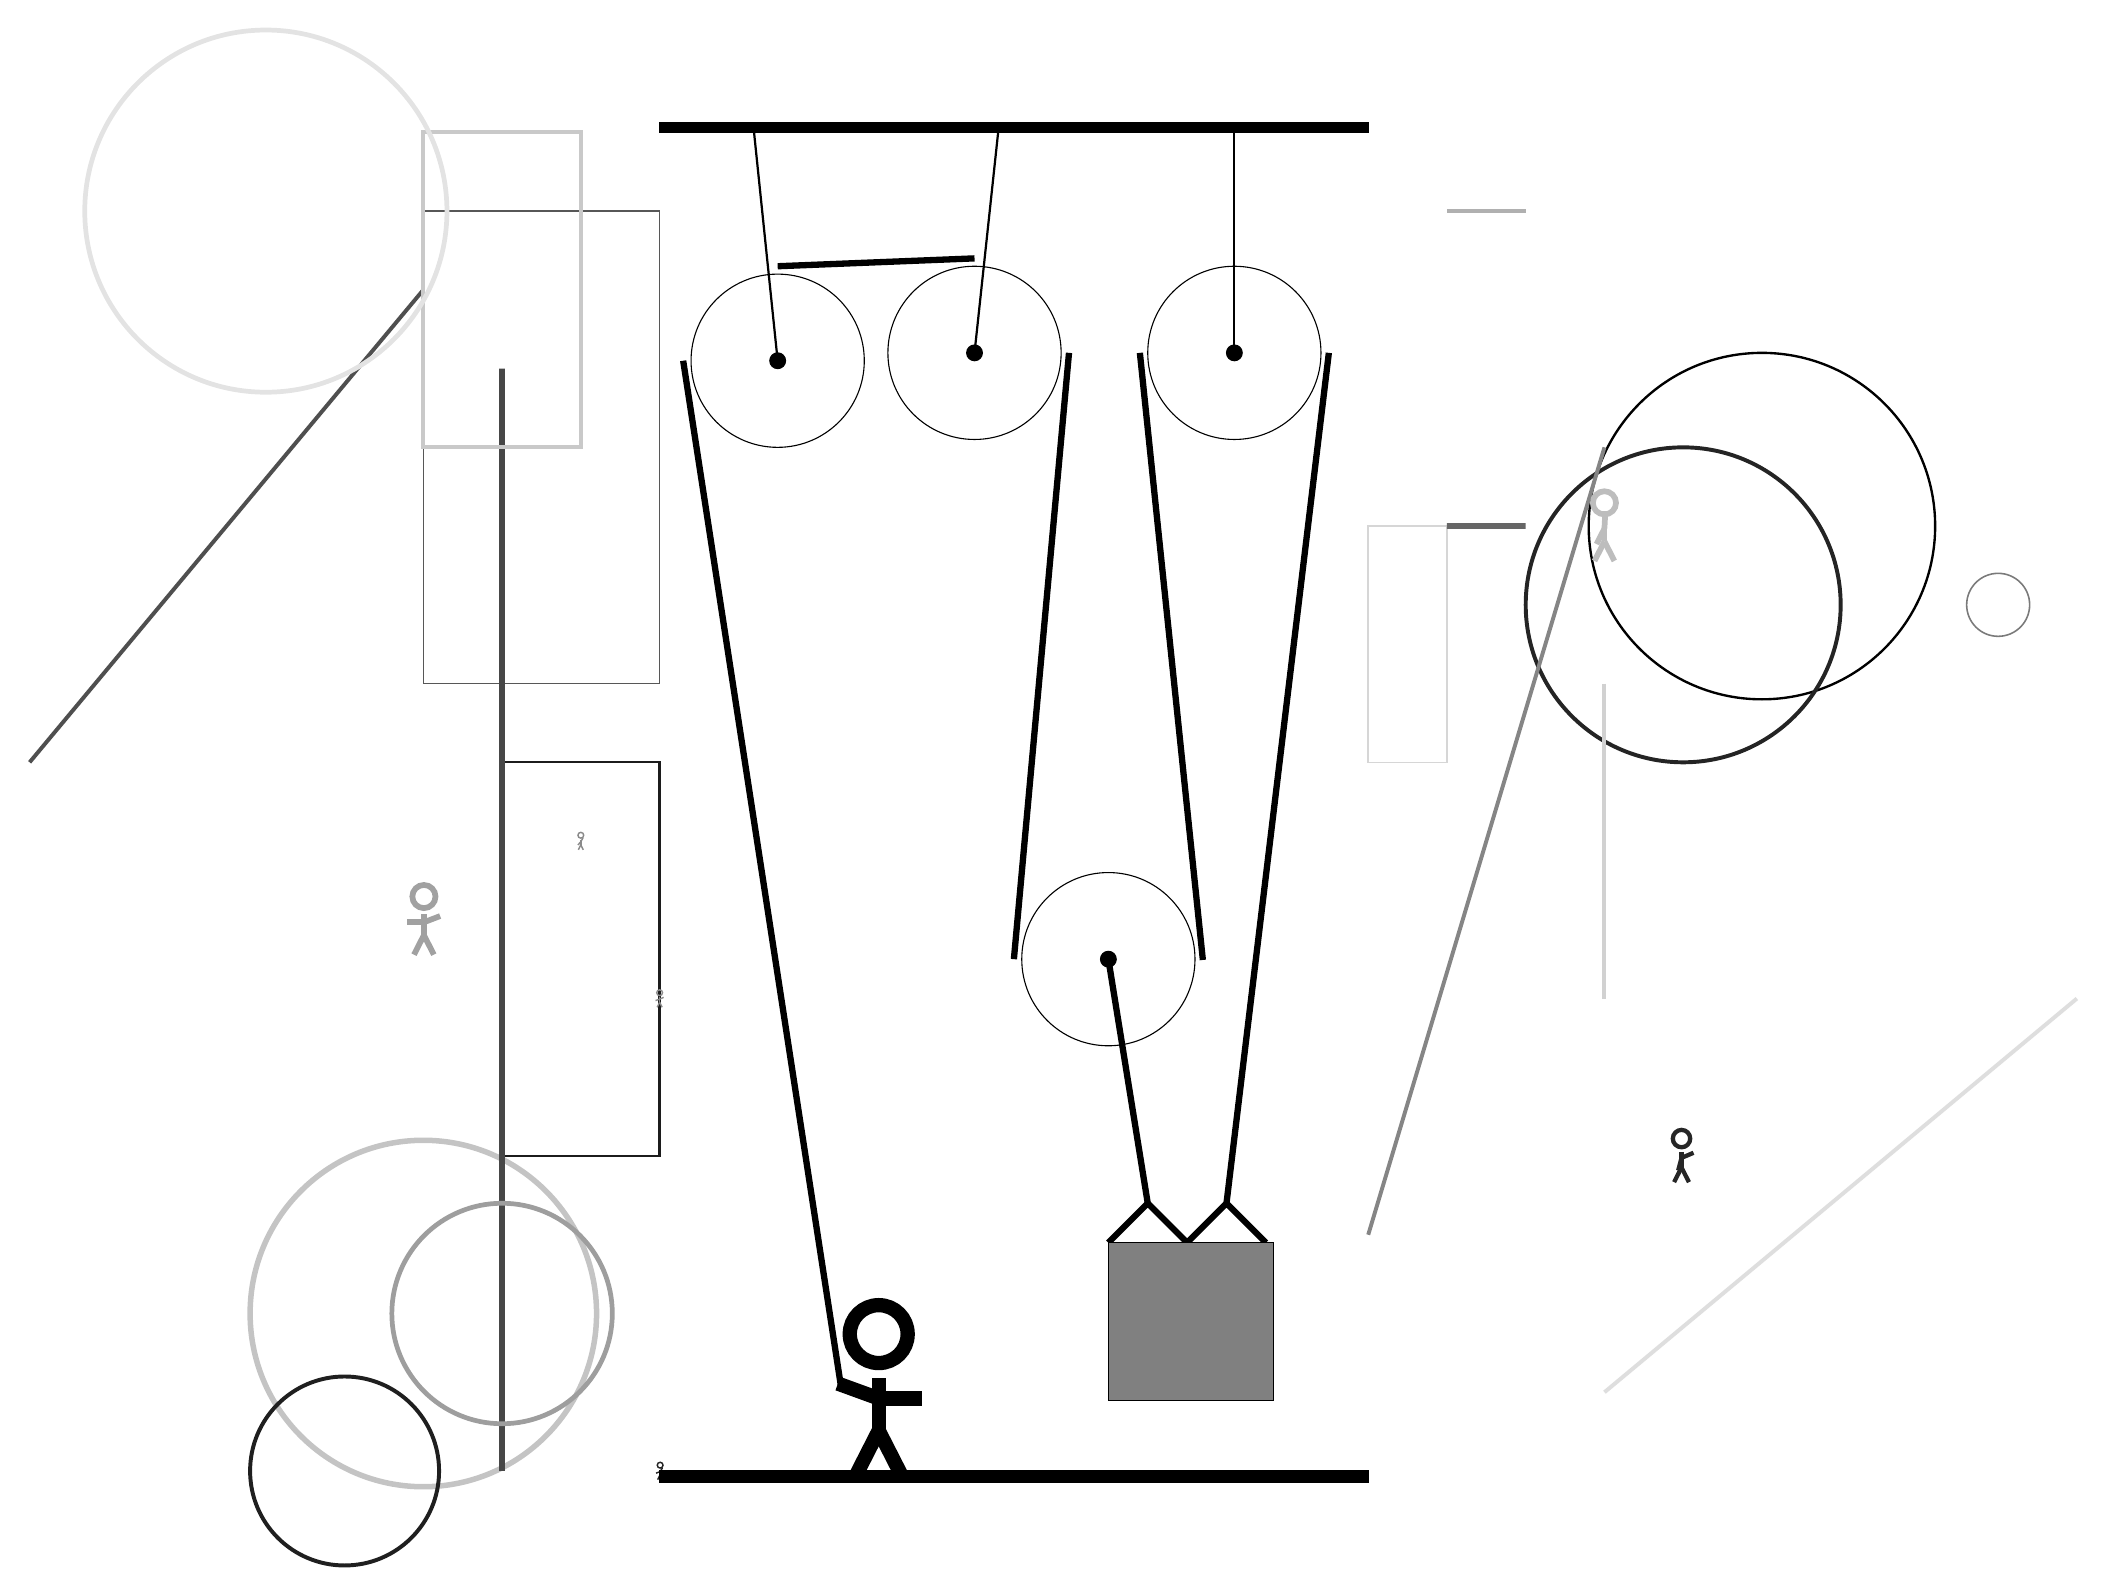
\begin{tikzpicture}
			%%%%% START %%%%%
			
			\draw[fill=black] (-3, 14) rectangle (6, 14.125);
			
			\draw[line width=0.2mm, color=black!16] (6, 6) rectangle (7, 9);
			
			\draw [line width=0.3mm, color=black!100](11, 9) circle (2.2);
			\node[line width=0.5mm, color=black!46] at (-4, 5) {\Strichmaxerl[1][49][60]};
			\draw[line width=0.2mm, color=black!66] (-3, 13) rectangle (-6, 7);
			
			\draw[line width=0.5mm, color=black!13](9, -2) -- (15, 3);
			\node[line width=0.4mm, color=black!86] at (-3, -3) {\Strichmaxerl[1][21][58]};
			\draw [line width=0.7mm, color=black!23](-6, -1) circle (2.2);
			\node[line width=0.2mm, color=black!85] at (10, 1) {\Strichmaxerl[3][75][23]};
			\draw[line width=0.3mm, color=black!89] (-5, 1) rectangle (-3, 6);
			
			\draw[line width=0.7mm, color=black!60] (8, 9) rectangle (7, 9);
			\draw [line width=0.5mm, color=black!86](10, 8) circle (2.0);
			
			\draw[line width=0.5mm, color=black!69](-6, 12) -- (-11, 6);
			\node[line width=0.6mm, color=black!37] at (-6, 4) {\Strichmaxerl[4][0][21]};
			\draw[line width=0.5mm, color=black!33] (-5, -1) rectangle (-5, -2);
			\draw[line width=0.7mm, color=black!72] (-5, -3) rectangle (-5, 11);
			\draw[line width=0.5mm, color=black!48](6, 0) -- (9, 10);
			
			\node[line width=0.7mm, color=black!26] at (9, 9) {\Strichmaxerl[4][63][87]};
			\draw[line width=0.5mm, color=black!21] (-4, 14) rectangle (-6, 10);
			\node[line width=0.3mm, color=black!45] at (-3, 3) {\Strichmaxerl[1][19][25]};
			\draw [line width=0.6mm, color=black!38](-5, -1) circle (1.4);
			\draw[line width=0.5mm, color=black!18](9, 7) -- (9, 3);
			
			\draw[line width=0.5mm, color=black!31](8, 13) -- (7, 13);
			
			\draw [line width=0.2mm, color=black!52](14, 8) circle (0.4);
			\draw [line width=0.6mm, color=black!11](-8, 13) circle (2.3);
			\draw [line width=0.5mm, color=black!88](-7, -3) circle (1.2);
			
			\draw (1, 11.2) circle (1.1);
			\draw[fill=black] (1, 11.2) circle (0.1);
			\draw[thick] (1, 11.2) -- (1.3, 14);
			
			\draw (4.3, 11.2) circle (1.1);
			\draw[fill=black] (4.3, 11.2) circle (0.1);
			\draw[thick] (4.3, 11.2) -- (4.3, 14);
			
			\draw (2.7, 3.5) circle (1.1);
			\draw[fill=black] (2.7, 3.5) circle (0.1);
			
			\draw[line width=0.8mm]  (2.7, -0.1) -- (3.2, 0.4) -- (3.7, -0.1) -- (4.2, 0.4) -- (4.7, -0.1);
			\draw[fill=black!50] (2.7, -0.1) rectangle (4.8, -2.1);
			
			\draw (-1.5, 11.1) circle (1.1);
			\draw[fill=black] (-1.5, 11.1) circle (0.1);
			\draw[thick] (-1.5, 11.1) -- (-1.8, 14);
			
			\draw[line width=0.8mm](-0.7, -1.9) --  (-2.7, 11.1);
			\centerarc[line width=0.8mm](-1.5, 11.1)(90:180:1.2000000000000002);
			\draw[line width=0.8mm](-1.5, 12.3) -- (1, 12.4);
			\centerarc[line width=0.8mm](1, 11.2)(0:90:1.2000000000000002);
			\draw[line width=0.8mm](2.2, 11.2) -- (1.5, 3.5);
			\centerarc[line width=0.8mm](2.7, 3.5)(180:370:1.2000000000000002);
			\draw[line width=0.8mm] (3.9, 3.49) -- (3.1, 11.2);
			\centerarc[line width=0.8mm](4.3, 11.2)(0:180:1.2000000000000002);
			\draw[line width=0.8mm](4.2, 0.4) -- (5.5, 11.2);
			\draw[line width=0.8mm] (3.2, 0.4) -- (2.7, 3.5);
			
			\node at (-0.2, -2) {\Strichmaxerl[10][-20][0]};
			
			\draw[fill=black] (-3, -3) rectangle (6, -3.15);
			
			%%%%% END %%%%%
		\end{tikzpicture}
	\end{figure}	
\end{document}